\documentclass[]{article}
\usepackage{lmodern}
\usepackage{amssymb,amsmath}
\usepackage{ifxetex,ifluatex}
\usepackage{fixltx2e} % provides \textsubscript
\ifnum 0\ifxetex 1\fi\ifluatex 1\fi=0 % if pdftex
  \usepackage[T1]{fontenc}
  \usepackage[utf8]{inputenc}
\else % if luatex or xelatex
  \ifxetex
    \usepackage{mathspec}
  \else
    \usepackage{fontspec}
  \fi
  \defaultfontfeatures{Ligatures=TeX,Scale=MatchLowercase}
\fi
% use upquote if available, for straight quotes in verbatim environments
\IfFileExists{upquote.sty}{\usepackage{upquote}}{}
% use microtype if available
\IfFileExists{microtype.sty}{%
\usepackage{microtype}
\UseMicrotypeSet[protrusion]{basicmath} % disable protrusion for tt fonts
}{}
\usepackage[margin=1in]{geometry}
\usepackage{hyperref}
\hypersetup{unicode=true,
            pdftitle={stan MCMC vs.~variational bayes: Consistency},
            pdfauthor={Ben Smith},
            pdfborder={0 0 0},
            breaklinks=true}
\urlstyle{same}  % don't use monospace font for urls
\usepackage{longtable,booktabs}
\usepackage{graphicx,grffile}
\makeatletter
\def\maxwidth{\ifdim\Gin@nat@width>\linewidth\linewidth\else\Gin@nat@width\fi}
\def\maxheight{\ifdim\Gin@nat@height>\textheight\textheight\else\Gin@nat@height\fi}
\makeatother
% Scale images if necessary, so that they will not overflow the page
% margins by default, and it is still possible to overwrite the defaults
% using explicit options in \includegraphics[width, height, ...]{}
\setkeys{Gin}{width=\maxwidth,height=\maxheight,keepaspectratio}
\IfFileExists{parskip.sty}{%
\usepackage{parskip}
}{% else
\setlength{\parindent}{0pt}
\setlength{\parskip}{6pt plus 2pt minus 1pt}
}
\setlength{\emergencystretch}{3em}  % prevent overfull lines
\providecommand{\tightlist}{%
  \setlength{\itemsep}{0pt}\setlength{\parskip}{0pt}}
\setcounter{secnumdepth}{0}
% Redefines (sub)paragraphs to behave more like sections
\ifx\paragraph\undefined\else
\let\oldparagraph\paragraph
\renewcommand{\paragraph}[1]{\oldparagraph{#1}\mbox{}}
\fi
\ifx\subparagraph\undefined\else
\let\oldsubparagraph\subparagraph
\renewcommand{\subparagraph}[1]{\oldsubparagraph{#1}\mbox{}}
\fi

%%% Use protect on footnotes to avoid problems with footnotes in titles
\let\rmarkdownfootnote\footnote%
\def\footnote{\protect\rmarkdownfootnote}

%%% Change title format to be more compact
\usepackage{titling}

% Create subtitle command for use in maketitle
\newcommand{\subtitle}[1]{
  \posttitle{
    \begin{center}\large#1\end{center}
    }
}

\setlength{\droptitle}{-2em}
  \title{stan MCMC vs.~variational bayes: Consistency}
  \pretitle{\vspace{\droptitle}\centering\huge}
  \posttitle{\par}
  \author{Ben Smith}
  \preauthor{\centering\large\emph}
  \postauthor{\par}
  \predate{\centering\large\emph}
  \postdate{\par}
  \date{9/27/2017}


\begin{document}
\maketitle

Variational Bayes is known to be less reliable than MCMC; my previous
analysis (compare\_models.Rmd) confirms that variational Bayes is less
reliable than we would like.

So the next step is to try the model again in MCMC. I'll repeat the
previous analysis, in which I repeatedly tested models with a couple of
different parameters, but this time, run it with both MCMC and
variational Bayes.

We want to answer the questions:

\begin{itemize}
\tightlist
\item
  For the reversal learning model, what is the speed like for MCMC
  compared to variational Bayes?
\item
  How much does MCMC improve our \emph{reliability} for an effect
  compared to variational Bayes?
\end{itemize}

\subsection{Settings}\label{settings}

One point which arose during this period was how much I had tried to
optimize variational Bayes. It might be that the iterations I used were
not enough. The default number of iterations for variational Bayes is
10000, but we had been using only 1000.

For an initial pilot analysis using the ``fastDebug'' option I created
which does just 100 iterations, the analysis duration was 1000 seconds.
For 4000 iterations (for MCMC), we can expect 40 times that duration, or
about 11 hours.

\section{Method}\label{method}

In the last comparison I tested out four different models. For this one,
I'll keep it simple, and just compare \texttt{double\_update.stan},
which processes only one run of reward \emph{or} punishment data. The
reason for this is that preliminary testing showed the full model was
not feasible to run on our system using MCMC (see later for details).

We'll run each model three times, as for the previous comparison. This
time we will be using MCMC rather than variational bayes to do the
estimation. We will also (as last time) run this for both Group 2 and
Group 3. All up, two groups, with two models, run three times, using two
different estimation techniques, this will require 24 repetitions.

In the backend, this has required some change to my \texttt{stan}
wrapper function:

\begin{itemize}
\tightlist
\item
  take a parameter which sets whether to use MCMC or variational bayes
  for an estimation task.
\item
  important for this analysis, we want to record the time taken for the
  analysis itself.
\item
  To improve reproduceability, I have set seed to a constant value for
  each iteration.
\end{itemize}

\section{Results}\label{results}

\subsection{Stan speed with Variational bayes and MCMC, and with and
without trial posterior
calculation}\label{stan-speed-with-variational-bayes-and-mcmc-and-with-and-without-trial-posterior-calculation}

It is important to optimize calculating models in RStan because it is
very computationally intensive. Initially, we were calculating trial
posteriors for each subject and trial in order to plot a predicted time
course for every subject. I tried our stan model script without that and
observed a marked improvement in processing time.

\begin{longtable}[]{@{}llrl@{}}
\toprule
model & estimation method & mean & range\tabularnewline
\midrule
\endhead
Basic double update with trial posteriors & vb & 116 & 98 to 131
s\tabularnewline
Basic double update with trial posteriors & MCMC & 13092 & 1613 to 20055
s\tabularnewline
Basic double update without trial posteriors & vb & 13 & 8 to 19
s\tabularnewline
Basic double update without trial posteriors & MCMC & 2517 & 451 to
10095 s\tabularnewline
\bottomrule
\end{longtable}

Across three iterations and two subject groups, calculated
independently, the basic double update model was consistently calculated
much faster using Variational Bayes, and generally faster when not
calculating trial posteriors.

If Variational Bayes is just as reliable as MCMC for this problem, there
would seem to be no reason to use MCMC, given Variational Bayes' speed.
Considering the difference between calculating without trial posteriors
and calculating with them, using Variational Bayes appears to be much
faster.

As can be seen across estimation methods and subject groups, calculation
was much faster when not calculating trial posteriors, so calculating
these shoul be avoided where it is not desirable.

\subsection{MCMC and Variational Bayes:
Reliability}\label{mcmc-and-variational-bayes-reliability}

\begin{figure}[htbp]
\centering
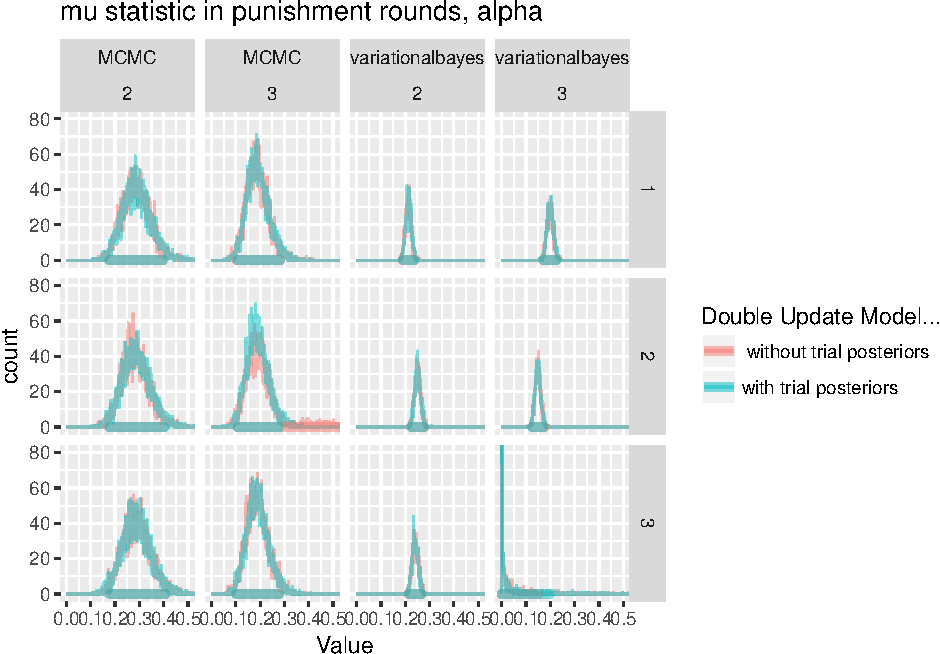
\includegraphics{compare_vb_and_MCMC_doubleUpdateOnly_files/figure-latex/VisualizeIterationConsistency-1.pdf}
\caption{TRUE}
\end{figure}

We set consistent speeds for each model configuration - randomization
seeds only differed between iterations. Figure
@ref(fig:VisualizeIterationConsistency) shows, as we would expect for a
correctly specified model and consistently set seeds, that including
trial posteriors generally made little difference to model estimations.
Each model does show some difference - likely random variation - and in
once case (the second iteration using MCMC to calculate a model for
Group 2), the model without trial posteriors produced a long tail not
observed in the model with trial posteriors.

Subsequent graphs in this section will present only results when not
calculating posteriors, unless otherwise specified.

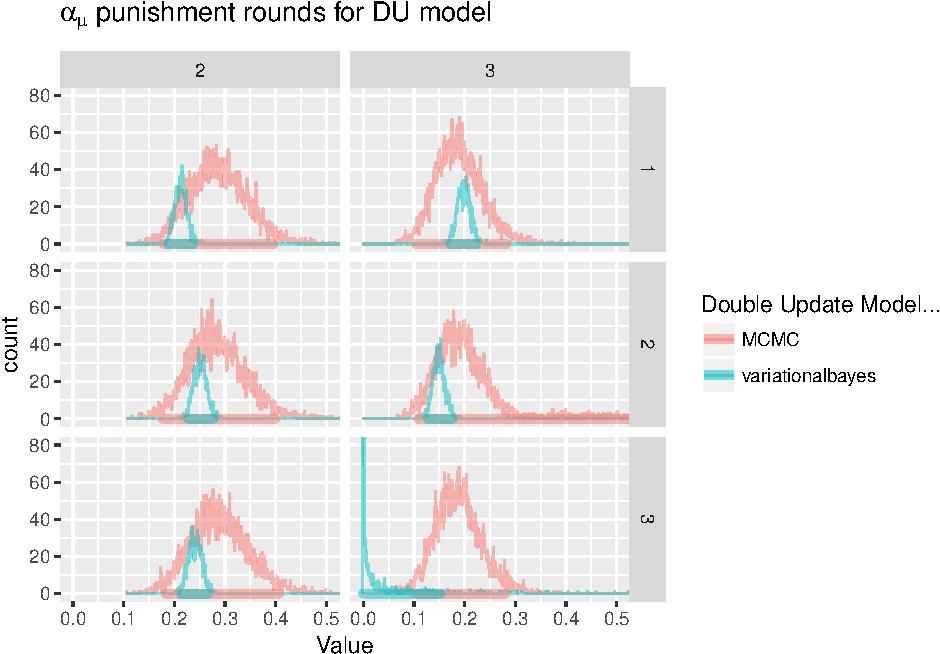
\includegraphics{compare_vb_and_MCMC_doubleUpdateOnly_files/figure-latex/CompareVBAndMCMCReliability-1.pdf}
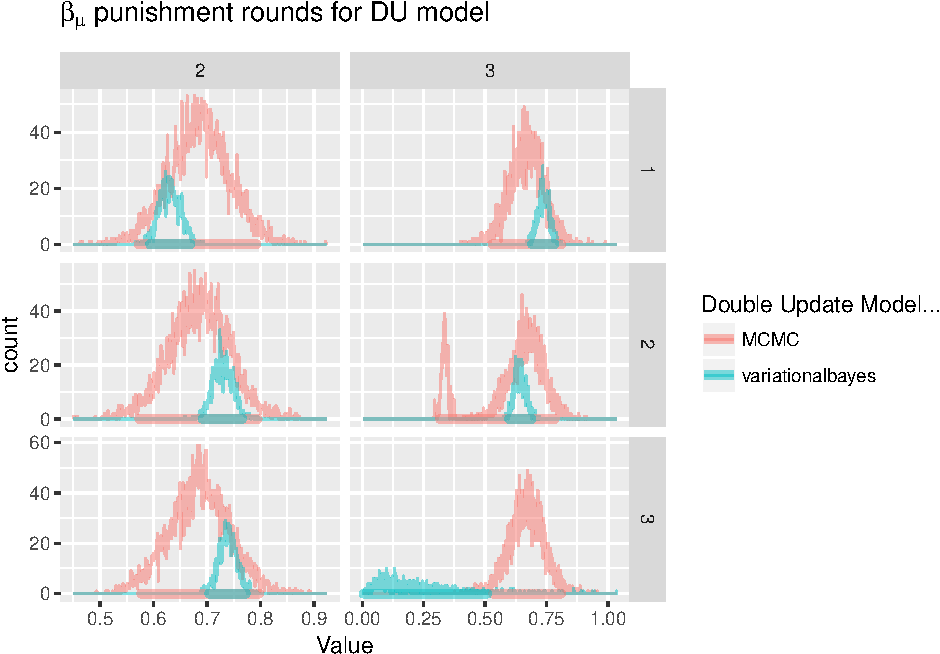
\includegraphics{compare_vb_and_MCMC_doubleUpdateOnly_files/figure-latex/CompareVBAndMCMCReliability-2.pdf}

From Figure @ref(fig:CompareVBAndMCMCReliability) it is immediately
apparent that MCMC, as we've applied it estimates much wider HDIs than
variational Bayes. We ran 2000 iterations: 1000 warmup iterations and
1000 estimation. It may be that estimation hadn't stabilized after 1000
steps, and we need to estimate more warmup iterations, and we may need
more estimation iterations, too. However, in most cases, MCMC estimates
seem to be relatively stable across iterations. That may be an
indication that the wide MCMC estimations correctly represent the data,
and that the true posterior distribution for these data are relatively
wide\footnote{A test of my randomization procedure suggested no problem with that (see seedtester.R)}.

Examining the Variational Bayes results, there are real concerns about
whether it has converged on appropriate results - it may be falling upon
local minima, as can be seen below:

\begin{figure}[htbp]
\centering
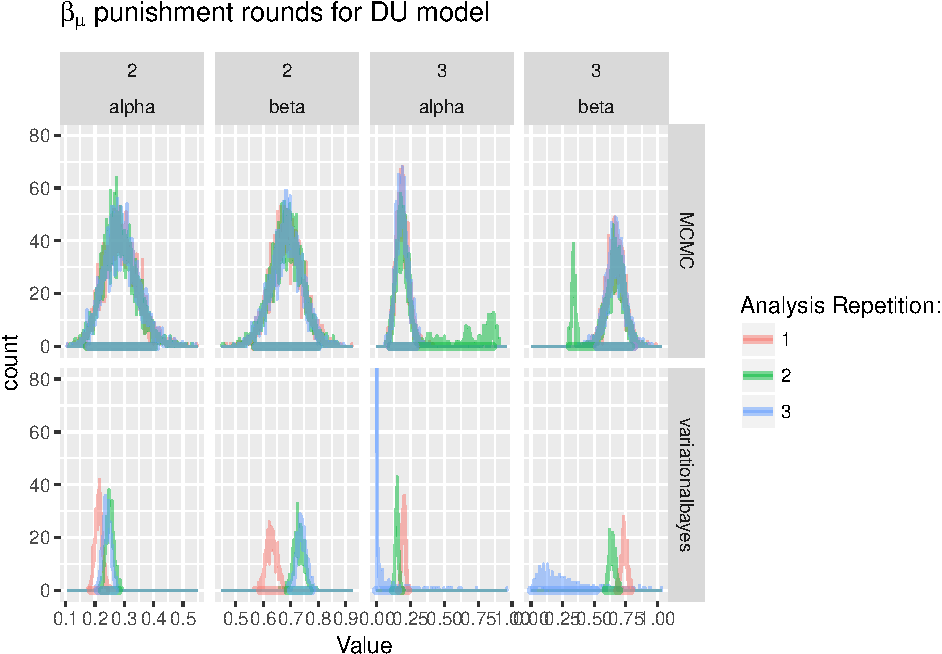
\includegraphics{compare_vb_and_MCMC_doubleUpdateOnly_files/figure-latex/CompareVBvsMCMCReliability2-1.pdf}
\caption{TRUE}
\end{figure}

The pattern here is that MCMC HDIs are much wider, but overlap from one
iteration to the next. In contrast, our Variational Bayes HDIs, across
repeated iterations, often entirely fail to overlap. Thus, it cannot be
assumed that our Variational Bayes calculations are reliable, whereas
our MCMC results, although they are insufficiently precise, seem to
accurately capture results, with one or two exceptions.

\subsection{MCMC Representativness, accuracy, and
efficiency}\label{mcmc-representativness-accuracy-and-efficiency}

Considering the wide HDIs produced by our MCMC estimates, I want to take
a closer look to see if the MCMC estimates are representative, accurate,
and efficient. \footnote{cite Kruschke}

\subsubsection{Representativeness}\label{representativeness}

To assess Representativeness for an MCMC algorithm, we need to see
whether chains have converged such that initial randomly-chosen priors
are not related to final values. We can visually examine the trace plots
below, and we can, examine teh density plots, and examine the
Gelman-Rubin statistic (Gelman \& Rubin, 1992) or the ``potential scale
reduction factor'' or ``shrink factor''. In \(rstan\), this is available
as the statistic \(\widehat{r}\).
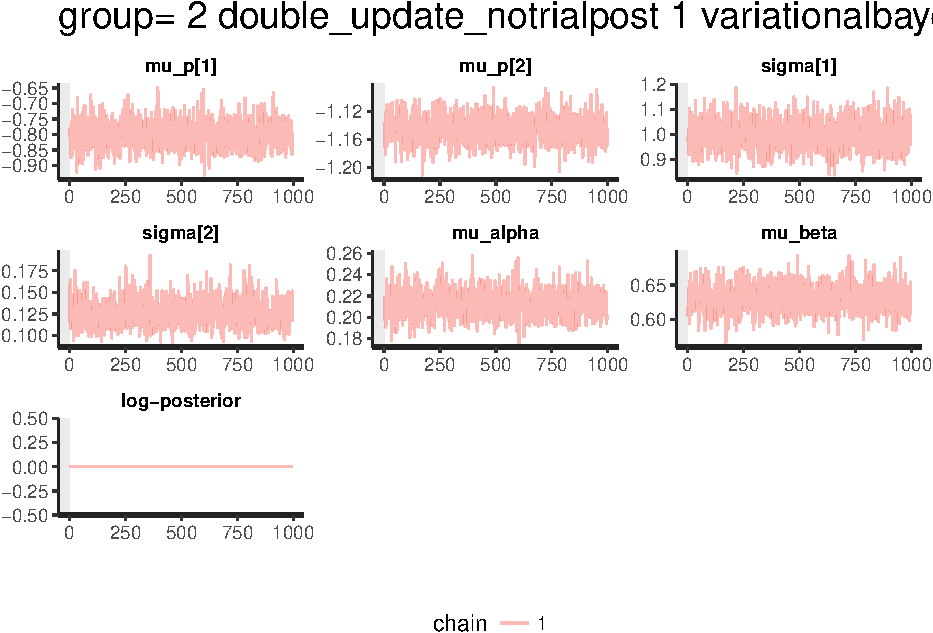
\includegraphics{compare_vb_and_MCMC_doubleUpdateOnly_files/figure-latex/StanTracePlot-1.pdf}
They look pretty stable, so we can't complain about instability, though
it is strange that there is such quick initial convergence followed by
stable but widely differing chain patterns.

For the double update (no trial posterior) version iteration 2, we do
see two parameters with one chain that failed to converge, although all
other chains converged correctly.

Do we see overlap of the chains, or do they not overlap very much? Given
the traceplot, I'd expect high levels of overlap.
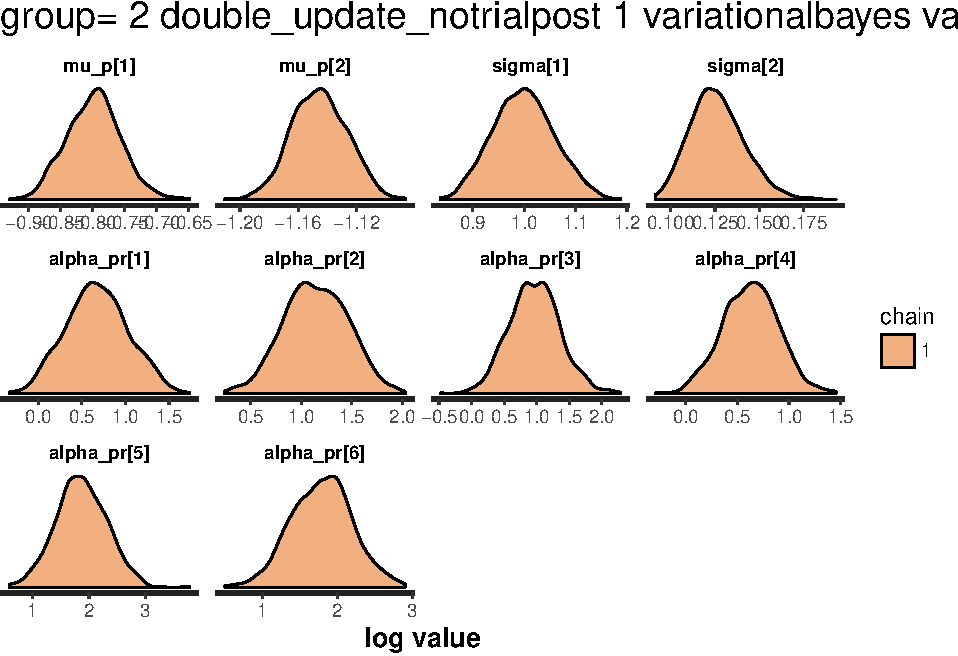
\includegraphics{compare_vb_and_MCMC_doubleUpdateOnly_files/figure-latex/StanPlotDensity-1.pdf}

Visually, these seem reasonably good, with the exception of Group 3, No
Trial Posteriors. How do we calculate MCSE and ESS?

\begin{verbatim}
## Inference for Stan model: double_update_notrialpost.
## 1 chains, each with iter=998; warmup=0; thin=1; 
## post-warmup draws per chain=998, total post-warmup draws=998.
## 
##           mean   sd  2.5%   25%   50%   75% 97.5%
## mu_p[1]  -0.80 0.04 -0.88 -0.83 -0.80 -0.77 -0.71
## mu_p[2]  -1.15 0.02 -1.18 -1.16 -1.15 -1.13 -1.11
## sigma[1]  1.00 0.06  0.89  0.96  1.00  1.04  1.12
## sigma[2]  0.13 0.02  0.10  0.12  0.13  0.14  0.16
## 
## Approximate samples were drawn using VB(meanfield) at Wed Oct  4 19:06:09 2017.
\end{verbatim}

the Rhat values, which are Brooks-Gelman-Rubin statistics or ``potential
scale reduction factors'' (Broooks \& Gelman, 1998; Kruschke, 20xx)
should be close to 1--and definitely within 10\% of 1 (0.91 to 1.1). It
appears that one MCMC failed to converge but others converged
separately.

\subsection{Accuracy}\label{accuracy}

To assess the \emph{accuracy} of the chains, we need to take into
account the \emph{effective sample size} (ESS)--how much independent
data actually exists in our analysis. To do this, we need a measure of
\emph{autocorrelation}. From ESS, we can get a measure of \emph{Monte
Carlo Standard Error}.

\subsubsection{Autocorrelation measures}\label{autocorrelation-measures}

We can view and measure autocorrelation in a number of ways: - To get
the effective sample size, we can use \texttt{rstan}'s
\texttt{stan\_ess}; bayesplot also offers
\href{\%5Bhttps://cran.r-project.org/web/packages/bayesplot/vignettes/visual-mcmc-diagnostics.html\#effective-sample-size}{appropriate
diagnostic tools}. Kruschke (20xx) recommends an effective sample size
of 10000 for estimating an HDI.

Kruschke advocates for an ESS of 10,000 for values like 95\% HDIs of
posteriors. Considering that we have 1000 post-warmup iterations and 6
chains, that equals 6000 iterations and ESS/SS appears to be in the
realm of 0.2-0.4. To get an ESS of 10,000, without optimizing the
function further, we'd need an actual sample size of 25,000 to 50,000.
Twelve chains of 4000 post-warmup iterations would get us 48,000, which
seems like a good amount to aim for.

\subsubsection{Monte Carlo Standard
Error}\label{monte-carlo-standard-error}

Monte Carlo Standard Error is calculated as

\[MCSE= ^{SD}/_{\sqrt{ESS}}\] or the standard formulation for standard
error, but with effective sample size used in place of actual sample
size.

We can view Monte Carlo Standard Error using the stan function
\texttt{stan\_mcse}.

\subsubsection{MCMC Efficiency}\label{mcmc-efficiency}

\emph{Efficiency} simply describes how efficient the estimation
algorithm is at calculating our model's result. This includes not only
measures like autocorrelation but also other model performance features
that could potentially slow it down.

Efficiency is one of Turner's key arguments for the use of DE-MCMC over
other forms of MCMC, such as the Metropolis-Hastings algorithm
(CITEREF:TURNER2013), or NUTS or Hamiltonian Markov Models (personal
communication) as implemented in Stan.

\section{Discussion}\label{discussion}

MCMC proved to yield stable results that, after a 1000-iteration
warm-up, with one notable exception, was representative, accurate, and
somewhat efficient. Compared to vb, it yielded posteriors that were
reliabile, but much less informative. Variational Bayes yielded
posteriors that seemed informative, but across repetitions, could be
shown to be completely unreliable.

Because variational Bayes is exponentially quicker - on the order of
only a few seconds--it may still be valuable to attempt to find reliable
results for variational Bayes.

The efficiency wasn't too bad; an \(ESS/SS\) ratio of between 0.2 and
0.4 seems acceptable, but falls well short of Kruschke's recommendation
for a sample size of around 10000 to estimate an HDI. Thus, the sample
size needs to be increased.

Increasing our sample size may also result in renegade chains, as was
observed for one iteration here, finally resolving.

Thus, from here, I need to:

\begin{itemize}
\tightlist
\item
  Run this again, using the full model
\item
  Run MCMC with a greater number of iterations - should be 12 chains and
  4000 post-warmup iterations. It will not be necessary to run more than
  2 analyses for each time, because the data here shows that across
  analyses, MCMC performance consistently estimated the value of key
  parameters.
\item
  Run Variational Bayes also with a greater number of iterations to see
  if it becomes more reliable.
\end{itemize}


\end{document}
